% !TEX TS-program = XeLaTeX
% use the following command:
% all document files must be coded in UTF-8
\documentclass[english]{textolivre}
% build HTML with: make4ht -e build.lua -c textolivre.cfg -x -u article "fn-in,svg,pic-align"

\journalname{Texto Livre}
\thevolume{15}
%\thenumber{1} % old template
\theyear{2022}
\receiveddate{\DTMdisplaydate{2022}{7}{13}{-1}} % YYYY MM DD
\accepteddate{\DTMdisplaydate{2022}{7}{27}{-1}}
\publisheddate{\DTMdisplaydate{2022}{8}{24}{-1}}
\corrauthor{Antonio Hernández Fernández}
\articledoi{10.35699/1983-3652.2022.40453}
%\articleid{NNNN} % if the article ID is not the last 5 numbers of its DOI, provide it using \articleid{} commmand 
% list of available sesscions in the journal: articles, dossier, reports, essays, reviews, interviews, editorial
\articlesessionname{dossier}
\runningauthor{Hernández Fernández} 
%\editorname{Leonardo Araújo} % old template
\sectioneditorname{Daniervelin Pereira}
\layouteditorname{Leonado Araújo}

\title{Neuropedagogy and neuroimaging}
\othertitle{Neuropedagogia e neuroimagem}
% if there is a third language title, add here:
%\othertitle{Artikelvorlage zur Einreichung beim Texto Livre Journal}

\author[1]{Antonio Hernández Fernández \orcid{0000-0002-7807-4363} \thanks{Email: \href{mailto:antonio.hernandez@ujaen.es}{antonio.hernandez@ujaen.es}}}
\affil[1]{Universidad de Jaén, Facultad de Humanidades y Ciencias de la Educación, Departamento Pedagogía, Jaén, España.}

\addbibresource{article.bib}
% use biber instead of bibtex
% $ biber article

% used to create dummy text for the template file
\definecolor{dark-gray}{gray}{0.35} % color used to display dummy texts
\usepackage{lipsum}
\SetLipsumParListSurrounders{\colorlet{oldcolor}{.}\color{dark-gray}}{\color{oldcolor}}

% used here only to provide the XeLaTeX and BibTeX logos
\usepackage{hologo}

% if you use multirows in a table, include the multirow package
\usepackage{multirow}

% provides sidewaysfigure environment
\usepackage{rotating}

% CUSTOM EPIGRAPH - BEGIN 
%%% https://tex.stackexchange.com/questions/193178/specific-epigraph-style
\usepackage{epigraph}
\renewcommand\textflush{flushright}
\makeatletter
\newlength\epitextskip
\pretocmd{\@epitext}{\em}{}{}
\apptocmd{\@epitext}{\em}{}{}
\patchcmd{\epigraph}{\@epitext{#1}\\}{\@epitext{#1}\\[\epitextskip]}{}{}
\makeatother
\setlength\epigraphrule{0pt}
\setlength\epitextskip{0.5ex}
\setlength\epigraphwidth{.7\textwidth}
% CUSTOM EPIGRAPH - END

% LANGUAGE - BEGIN
% ARABIC
% for languages that use special fonts, you must provide the typeface that will be used
% \setotherlanguage{arabic}
% \newfontfamily\arabicfont[Script=Arabic]{Amiri}
% \newfontfamily\arabicfontsf[Script=Arabic]{Amiri}
% \newfontfamily\arabicfonttt[Script=Arabic]{Amiri}
%
% in the article, to add arabic text use: \textlang{arabic}{ ... }
%
% RUSSIAN
% for russian text we also need to define fonts with support for Cyrillic script
% \usepackage{fontspec}
% \setotherlanguage{russian}
% \newfontfamily\cyrillicfont{Times New Roman}
% \newfontfamily\cyrillicfontsf{Times New Roman}[Script=Cyrillic]
% \newfontfamily\cyrillicfonttt{Times New Roman}[Script=Cyrillic]
%
% in the text use \begin{russian} ... \end{russian}
% LANGUAGE - END

% EMOJIS - BEGIN
% to use emoticons in your manuscript
% https://stackoverflow.com/questions/190145/how-to-insert-emoticons-in-latex/57076064
% using font Symbola, which has full support
% the font may be downloaded at:
% https://dn-works.com/ufas/
% add to preamble:
% \newfontfamily\Symbola{Symbola}
% in the text use:
% {\Symbola }
% EMOJIS - END

% LABEL REFERENCE TO DESCRIPTIVE LIST - BEGIN
% reference itens in a descriptive list using their labels instead of numbers
% insert the code below in the preambule:
%\makeatletter
%\let\orgdescriptionlabel\descriptionlabel
%\renewcommand*{\descriptionlabel}[1]{%
%  \let\orglabel\label
%  \let\label\@gobble
%  \phantomsection
%  \edef\@currentlabel{#1\unskip}%
%  \let\label\orglabel
%  \orgdescriptionlabel{#1}%
%}
%\makeatother
%
% in your document, use as illustraded here:
%\begin{description}
%  \item[first\label{itm1}] this is only an example;
%  % ...  add more items
%\end{description}
% LABEL REFERENCE TO DESCRIPTIVE LIST - END


% add line numbers for submission
%\usepackage{lineno}
%\linenumbers

%\usepackage{array}
%\usepackage{makecell}

\begin{document}
\maketitle

\begin{polyabstract}
\begin{abstract}
The present study is based on the assumption that there is a lack of information, both nationally and internationally, on neuropedagogy, and that there is more than enough evidence of the need for a conceptualization of neuropedagogy. Therefore, the general objective is to analyze the relationship between neuroeducation, neurodidactics, teacher training and neuropedagogy. Data collection was carried out with a 27-item ad hoc Likert scale questionnaire, reliable (Cronbach's Alpha, .973), and validated in its content and construct with an exploratory factor analysis (KMO (.843), Bartlett (Sign.000), Determinant (9.416E-19)). The research sample was selected by convenience from among university teachers in Spain, Paraguay, Ecuador, Brazil and Mexico, with a total of 1264 participants. The research design is non-experimental, descriptive, explanatory, correlational and regression-based. The results show that the future of pedagogy must include neuropedagogy, evidencing: 1) the need of neuroeducation knowledge for Neuropedagogy; 2) the understanding of neurodidactics as the practical application for neuropedagogy, 3) the importance of neuro-orientation and neuro-educational organization, and 4) the need for the training of trainers. All of which is reinforced by the examples shown of neuroimaging that demonstrate the need for neuropedagogy and teacher training in neuropedagogy.

\keywords{Neuropedagogy \sep Neuroimaging \sep Pedagogy \sep Teaching \sep Brain}
\end{abstract}

\begin{portuguese}
\begin{abstract}
A pesquisa aqui apresentada se baseia no pressuposto de que existe uma falta de informação, tanto nacional como internacional, sobre a neuropedagogia, e que há provas mais do que suficientes da necessidade de uma conceitualização da neuropedagogia. Por essa razão, o objetivo geral é analisar a relação entre neuroeducação, neurodidática, treinamento de professores e neuropedagogia. A coleta de dados foi realizada utilizando um questionário \textit{ad hoc} de escala Likert de 27 itens, confiável (Cronbach's Alpha, .973) e validado em termos de conteúdo e construção com uma análise exploratória de fatores (KMO (.843), Bartlett (Sign.000), Determinant (9.416E-19)). A amostra da pesquisa foi selecionada por conveniência entre professores universitários na Espanha, Paraguai, Equador, Brasil e México, com um total de 1264 participantes. O desenho da pesquisa é não-experimental, descritivo, explicativo, correlacional e regressivo. Os resultados mostram que o futuro da pedagogia deve incluir a neuropedagogia, evidenciando que a neuropedagogia precisa do conhecimento da neuroeducação, que a neurodidática é a aplicação prática da neuropedagogia, a importância da neuroorientação e da neuro-organização na educação, e a necessidade de treinamento de instrutores. Tudo isso é reforçado pelos exemplos mostrados de neuroimagem que demonstram a necessidade de neuropedagogia e treinamento de professores em neuropedagogia.

\keywords{Neuropedagogia \sep Neuroimagem \sep Pedagogia \sep Professor \sep Cérebro}
\end{abstract}
\end{portuguese}
% if there is another abstract, insert it here using the same scheme
\end{polyabstract}

\section{Introduction}\label{sec-intro}
Each principle is the ideal moment to realize that the balances are established in the most accurate way \cite{herbert_dune_1965}, in the subject addressed in this study, this balance is key, because we are dealing with a very delicate subject. The topic of de present study is neuropedagogy, which we are going to address both theoretically and empirically, as well as to illustrate from neuroimaging. We begin by reviewing the research topics.

The first topic is neuroscience, which is an area of knowledge that focuses on studying the structure and functioning of the nervous system, as well as the interaction of brain elements that give rise to the behavior of human beings \cite{blakemore_como_2007,manes_usar_2014}, in order to understand how thought, consciousness, social interaction, creativity, perception, free will, emotion, among other facts, originate, which leads to the multidisciplinary nature of this new science. It must bring together neurologists, psychologists, psychiatrists, philosophers, linguists, biologists, engineers, physicists and mathematicians \cite{manes_usar_2014}, as well as physicians, sociologists, theologians and a long list of others specialist, since understanding brain functioning is everyone's responsibility \cite{cumpa_valencia_usos_2019}. Neuroscience applied to education is the basis of neuroeducation, the second topic of study, as a discipline that aims to develop new teaching and learning methods combining pedagogy, neurobiology and cognitive sciences \cite{manes_usar_2014}. Neuroeducation is configured as a branch of education, which links knowledge based on neuroimaging with the way the brain interacts with its environment. Specifically, it focuses on the learning/teaching process. A new persepctive at the school process that links Neuroscience and Education \cite{bejar_neuroeducacion_2014}.

On the other hand, to speak of neuropedagogy requires first defining the concept of pedagogy and its field of action. Etymologically, the word pedagogy comes from two Greek roots: paidós = child, and ago = I lead. This gave rise to the term pedagogue, who was the slave in charge of taking children to the master responsible for teaching. By extension, pedagogue has become synonymous with teacher or preceptor, this term being used in the seventeenth and eighteenth centuries to designate the preceptors of wealthy families. Gradually the word extended its former meaning, coming to be understood not as corresponding to the act of conducting but to that of regulating the whole process of education. The French Academy admitted it in 1762 and \textcite{durkheim_jugements_1911} defines Pedagogy as the practical theory of education. For many centuries, pedagogical ideas were mixed with philosophical, religious or political ideas. This occurs in the Instituciones Oratorias, by Quintiliano, which is, according to Rufino Blanco, the first treatise on pedagogy; “Erudito Didascalia”, by Rugo de San Victor; “Tratado de la Enseñanza”, by Luis Vives; “Didáctica Magna”, by Comenio, and “El Emilio”, by Rousseau. It is necessary to arrive at Herbart and his work General Pedagogy derived from the end of Education, published in 1806, to find a well-founded systematization and the proper use of the term Pedagogy. Subsequently, its meaning has been enriched. Positivism questions the possibility of a philosophical foundation of pedagogy and widens the field of its possibilities with the incorporation of historical and experimental methods. Neoidealism understands that pedagogy is not independent of philosophy, and thus addresses the issue of its autonomy. Nowadays, experimental, historical and comparative methods are being studied in depth. Their studies cannot be understood without recourse to psychology, sociology, statistics or cybernetics. The pedagogical fact cannot be explained except through interdisciplinarity \cite[p. 12-18]{rotger_amengual_ciencias_1984}.

According to Gaston Mialaret, it is necessary to go back to 1960 to establish a clear distinction between the terms Pedagogy and Education. Education is a palpable reality, a living process, a concrete activity. It gives rise to problems to be overcome, theories and doctrines, norms and principles of action. Pedagogy is the discipline, education the effectiveness. Pedagogy belongs to the category of reflection; education to that of action. Pedagogy is the discipline; education, its proper object. However, they cannot be absolutely separated, since, like action and thought, they are two things similar. The structure of pedagogy cannot be understood if the concept of education is not understood. Educare means to bring up, to nourish; exducere or educere, to bring out, to bring to. The analysis of both etymologies can lead to two historically distinct and ideologically opposed interpretations, thus educare: to raise, to feed, from the outside to the inside, principal agent, passive, receiver, person to be trained, directive, systematization, instruction, authority, discipline, receptivity, traditional and conservative. Educere: to take out, to take to..., from the inside to the outside, guide and stimulator, person to be formed, non-directive, originality, creativity, autonomy, freedom, active response, new, progressive \cite[p.8]{rotger_amengual_ciencias_1984}. Likewise, it is important to know the bases that configure Pedagogy, for this, following \textcite{sarramona_aspectos_1977}, the division of Pedagogy can be made from three points of view: 1.-Foundation (Aims; Transcendent (Theology of education); Immanent (Philosophy of education)); Conditional; Personal (Biology of education, Psychology of education) and Social (Sociology of education, Economics of education)). Normative (Historical (History of education); Geographical (Comparative education); General (General pedagogy) and Differential (Differential pedagogy). 3.-Application (Educational (Educational guidance); School environment (School organization) and Instructional (Didactics)).

Finally, in relation to the topic "Neuropedagogy" a search was carried out in the Scopus database, with the entries "neuropedagogy" and "neuro pedagogy", with no results. From the searches carried out in Google Scholar and other databases, once the articles had been debugged and the appropriate information for this research had been extracted, we highlight three authors. First, \textcite{jimenez_ludica_2010} expresses that for Neuropedagogy the object of study is the life of man, and especially his brain, understood not as a computer, but as a social organ that needs embrace, recreation and play for its development (p. 2). For \textcite{castillo_neurociencias_2015} neuropedagogy arises from the union of pedagogy, psychology and neuroscience; in an effort to study the brain and its functions, to approach man integrally from a social dimension, recognizing his needs and characteristics to potentiate them and develop multiple aspects, including learning. When we talk about neuropedagogy we refer to how the brain works, and how brain understanding can be used to explain the favoring or not of children's learning practices. Finally, \textcite{torres_rios_caracterizacion_2018} posit that neuropedagogy allows teachers to improve their students' learning. In this sense, they consider that university teachers need to know about this discipline in order to design didactic strategies that allow students the formation of the competencies contained in the curriculum of their career.

We end with the topic "neuroimaging". Neuroimaging techniques allow visualizing live images of the brain, being the electroencephalogram one of the most used techniques in neuroimaging. Neurons generate electricity, which passes through the skull and can be measured on the outside of the head. The waves generated by the brain are characteristic, thus \textcite{cardinali_neurociencia_2007} establishes five main frequency bands: delta (less than 4Hz), theta (4 to 8 Hz), alpha (8 to 12 Hz), beta (14 to 30Hz) and gamma (30 to 80 Hz). It should be noted that all emotions, thoughts and actions are possible thanks to brain waves, hence their importance and relevance in neuropedagogical studies. In this research, we have used the 14-channel emotiv epoc+ brain computer interface (BCI) to exemplify future guidelines for neuroimaging studies in neuropedagogy. This system has fourteen EEG readout channels and two reference sensors, as well as a two-axis gyroscopic sensor that is designed for advanced practical and in-context research for BCIs. It provides access to raw data, also known as primary data or Raw data, of high quality and high spectral density, i.e. where the signals present high power or energy \cite[p. 23]{cardenas_gomez_identificacion_2021}.

In the current literature we do not find research like the one presented here, which basically tries to show the role of neuropedagogy in the current scientific context, establishing the parameters as a teaching discipline in pedagogical studies, and exemplifying, in a practical way, how to use neuroimaging in this research context.

\section{Method}\label{sec-normas}
This research has as its main goal to analyze the relationship between neuroeducation, neurodidactics, teacher training and neuropedagogy. It is based on a non-experimental, descriptive, explanatory and correlational design, with a quantitative methodology. The research instrument used is a Likert scale questionnaire constructed ad hoc. The study dimensions established are: A.-Neuroeducation, B.-Neuropedagogy, C.-Neurodidactics and D.-Teacher training. The dependent variable is Neuropedagogy, the independent variables are: neuroeducation, neurodidactics and teacher training.

The sample was made by convenience among professors from universities in Spain, Paraguay, Ecuador, Brazil and Mexico, with an academic degree of master's and/or doctorate and professional category of hired doctor, tenured university professor or professor. The total sample consisted of 1264 participants, of whom 527 were from Spain, 512 from Paraguay, 54 from Ecuador, 115 from Brazil and 56 from Mexico.

The data collection instrument was constructed with the corresponding operationalization table, with a total of 27 items. The content validity was carried out with a judgment of 12 experts (K coefficient of .9) and a final pilot test, where, after the suggestions of the judges and the pilot test, the instrument was considered validated in its content. Reliability was calculated with Cronbach's Alpha, with a result of .973, which is excellent \cite{george_spss_2003}.

\section{Results}\label{sec-conduta}
The initial results are drawn from the construct validity, which was performed through exploratory factor analysis, following the steps of \textcite{garcia_ferrando_alisis_2015}.

1. Study of the correlation matrix: it is necessary to study the correlation matrix to check if our data are suitable to carry out a Factorial Analysis. To do this, this matrix must have a certain structure. To check this, we have used the Kaiser-Meyer-Olkin measure of sampling adequacy (KMO coefficient), in our case the value is of KMO is 0.843, following \textcite{kaiser_index_1974} the value is adequate, the result of Bartlett's sphericity test is .000 and the determinant 9.416E-19, so we continued with the analysis.

2. Extraction of the factors: once it was decided that the factorial analysis my provide suitable results, the extraction of the factors is carried out. In a good extraction these values should be high (the closer to one the better) in all variables. The resulting of communalities showed us that the factors have a value greater than .492 so it was not necessary to eliminate any item from the factor analysis.

The best represented items are: D26.-Teacher training in practical neuropedagogical aspects is necessary (.943); D23.-Teacher training in neuropedagogy is necessary (.940) and D25.-Teacher training in theoretical neuropedagogical aspects is necessary (.930). The worst rated item is A5.-Neuroeducation provides the theoretical basis for neuropedagogy (.492).

3-Rotation of the factors: To carry out the rotations there are several methods according to the criterion of optimality. One of them is the Varimax Rotation which optimizes the factorial loads so that the most extreme loads are obtained in the factors (high and low). There are rules to know the most adequate number of factors to conserve, for example, the one known as \posscite{kaiser_index_1974} criterion, which indicates that it is necessary to conserve the main components whose own values are greater than the unit, although the most used criterion is that of observing the percentage of total variance explained by each component or factor, and when this reaches an accumulated percentage considered high, in our case they are the first 4 factors, which explain 76,650\% of the accumulated variance.

4 - Study of factorial scores: \Cref{tab01} shows the analysis of variance explained and accumulated, as well as the determination of factors and distribution of items according to the highest level of saturation by factors (we have discarded the factors that have less than three items, leaving only two factors that may have an acceptable reliability).


\begin{table}[h!]
\begin{threeparttable}
\caption{Analysis of variance explained and accumulated.}
\label{tab01}
\centering
\begin{tabular}{p{0.8cm} p{1.5cm} p{1.5cm} p{9.1cm}}
%\begin{tabular}{m{1em} m{1em} p{1.5cm} p{8.5cm}}
%\begin{tabularx}{\textwidth}{lllX}
\toprule
Factor & Title & \% of cumulative variance & Items integrated in each factor of the questionnaire \\
\midrule
\multirow{4}{*}{I} & 
A \newline (Neuro\-education) & 
\multirow{4}{*}{20,486 \%} & 
A1.-The application of neuroscientific bases to the educational context is a necessity.

A2.-The study of the brain and neurotransmitters is important for teachers.

A3.-Neuromyths prevent a teacher from effective didactic performance.

A5.-Neuroeducation provides the theoretical basis for neuropedagogy. \\

 & B \newline(Neuro\-pedagogy) & & 
B6.-Pedagogy studies the human being in its educational facet.
 
B7.-Neuropedagogy studies the human being, in its educational facet, with a neuroscientific basis.

B8.-Neuropedagogy should be included in the curricula of university courses related to education.

B9.-The neurobiology of education is an important component of neuropedagogy.

B10.-The neurosociology of education is integrated into neuropedagogical studies.

B11.-Neuropedagogy has knowledge of comparative neuroeducation and differential neuropedagogy.

B12.-Educational neuro-orientation and school neuro-organization are key in neuropedagogical knowledge.

B13.-Neurodidactics is the instructional application of neuropedagogy in the classroom.

B14.-A new approach to research methodology in neuropedagogy is needed.

B15.-The field of knowledge of the Theory of Education must include neuropedagogy. \\

& C \newline (Neuro\-didactics) & & 
C16.-Neuropedagogy studies the optimization of teaching methodology with neuroscientific contributions.

C17.-Neurodidactics favors the creation of synapses and neuronal connections.

C18.-The study of the brain positively influences the didactic methodology of the teacher.

C19.-Neurotransmitters have a relevant role in the teaching-learning process.

C21.-The teaching methodology must have a didactic and neurodidactic base. \\

& D \newline (Teacher training) & & 

D22.-Teaching training in neuroeducation is necessary.

D23.-Teaching training in neuropedagogy is necessary.

D24.-Teaching training in neurodidactics is necessary.

D25.-Teacher training in theoretical neuropedagogical aspects is necessary.

D26.-Teaching training in practical neuropedagogical aspects is necessary.

D27.-Training of trainers in neuropedagogy is necessary.\\
\bottomrule
\end{tabular}
\source{Own elaboration}
\end{threeparttable}
\end{table}

We have calculated Cronbach's alpha of both factors: Factor 1: .974 (25 items), "excellent" rating. We took the factor 1, which presents a higher reliability than the original scale itself, getting a final scale of 27 items (.973), reducing 2 items.

To carry out the correlation, we subjected the Likert scale to the Kruskal-Wallis test, which explains that the data do not follow a normal distribution, so the Pearson correlation has to be used. Next we show the correlations between research dimensions that have significant value (0.05):
-Dimension A (Neuroeducation) correlates significantly with dimension B (Neuropedagogy).

-Dimension B (Neuropedagogy) correlates significantly with dimension C (Neurodidactics) and vice versa.

-Finally, dimension D (Teacher training) correlates significantly with dimension A (Neuroeducation).

Next, an automatic linear modeling was performed, for which Neuropedagogy was taken as a target, and the variable "country" as a weighting element of the analysis. The result shows a model with 100\% accuracy, which can be seen in \Cref{fig01}:
	
\begin{figure}[h!]
 \centering
 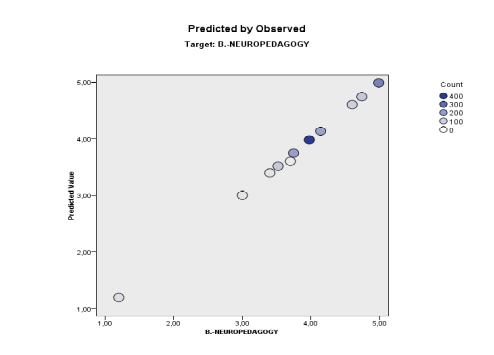
\includegraphics[width=0.85\textwidth]{Fig1.png}
 \caption{Predicted by observed.}
 \label{fig01}
 \source{Own elaboration.}
\end{figure}

For the prediction about Neuropedagogy to be fulfilled, we must take into account, as the most important aspect:
B11.-Neuropedagogy has knowledge of comparative neuroeducation and differential neuropedagogy. 

In decreasing order of importance:
\begin{description}
    \item[B7.]-Neuropedagogy studies the human being, in its educational facet, with a neuroscientific basis.
    \item[B13.]-Neuropedagogy is the instructional application of neuropedagogy in the classroom.
    \item[B12.]-Educational neuro-orientation and school neuro-organization are key to neuropedagogical knowledge.
    \item[B6.]-Pedagogy studies the human being in its educational facet.
    \item[B10.]-Neuro-sociology of education is integrated in neuropedagogical studies.
    \item[B15.]-The field of knowledge of the Theory of Education must include neuropedagogy.
    \item[A2.]-The study of the brain and neurotransmitters is important for teachers.
    \item[D27.]-Training of trainers in neuropedagogy is necessary.
    \item[B9.]-The neurobiology of education is an important component of neuropedagogy.
\end{description}


\section{Neuroimaging in neuropedagogy}\label{sec-fmt-manuscrito}
The neuropedagogical field needs the scientific basis provided by neuroimaging, which is the key to study, analyze and ultimately make visible the pedagogical processes that occur in real time in teachers and students in order to establish the neural networks of these processes and reach an education with a scientific-pedagogical basis of quality.

With all of the above, it is not about entering the medical or psychological field. On the contrary, it is about complementing it so that together we can provide teachers and student with guidelines; to achieve the greatest pedagogical potential the educational community.

The examples hereby shown require the person in charge of the BCI to 1) have neuroscientific, neuroeducational and neuropedagogical knowledge; 2) have a specific training in brain waves and their interpretation; 3) know the neurodidactic networks present in the pedagogical processes and 4) have the appropriate training for the use of the BCI \cite{hernandez_neuroimagen_2022}.

Next, we show the location of the BCI electrodes (\Cref{fig02}), as well as the placement of the emotiv (\Cref{fig03}) on the author. We begin the neuroimaging process by showing the brain function, extracted from a group of twenty-two children (8 years of age), randomly taken from an educational center, who is subjected to the following tasks, in his usual context: the children are reading three texts: 1) text and imagen (\Cref{fig04}); 2) text in script font (\Cref{fig05}); 4) foreign language (\Cref{fig06}); 5) arithmetic operations of addition (\Cref{fig07}); 6) subtraction (\Cref{fig08}); 7) multiplication (\Cref{fig09}); 8) division (\Cref{fig10}); 9) and a mathematical problem solving (\Cref{fig11}). In each case we will draw some appropriate neuropedagogical conclusions. As an example, the aim is not to draw general conclusions, nor standardized guidelines, which will be published in later works, but to show the lines of research that we are developing in the research groups EMIPE (University Autonomous of Madrid), ProfesioLab (University of Granada), and the University of Jaén in Spain.

\begin{figure}[htbp]
 \centering
 \begin{minipage}{.45\textwidth}
 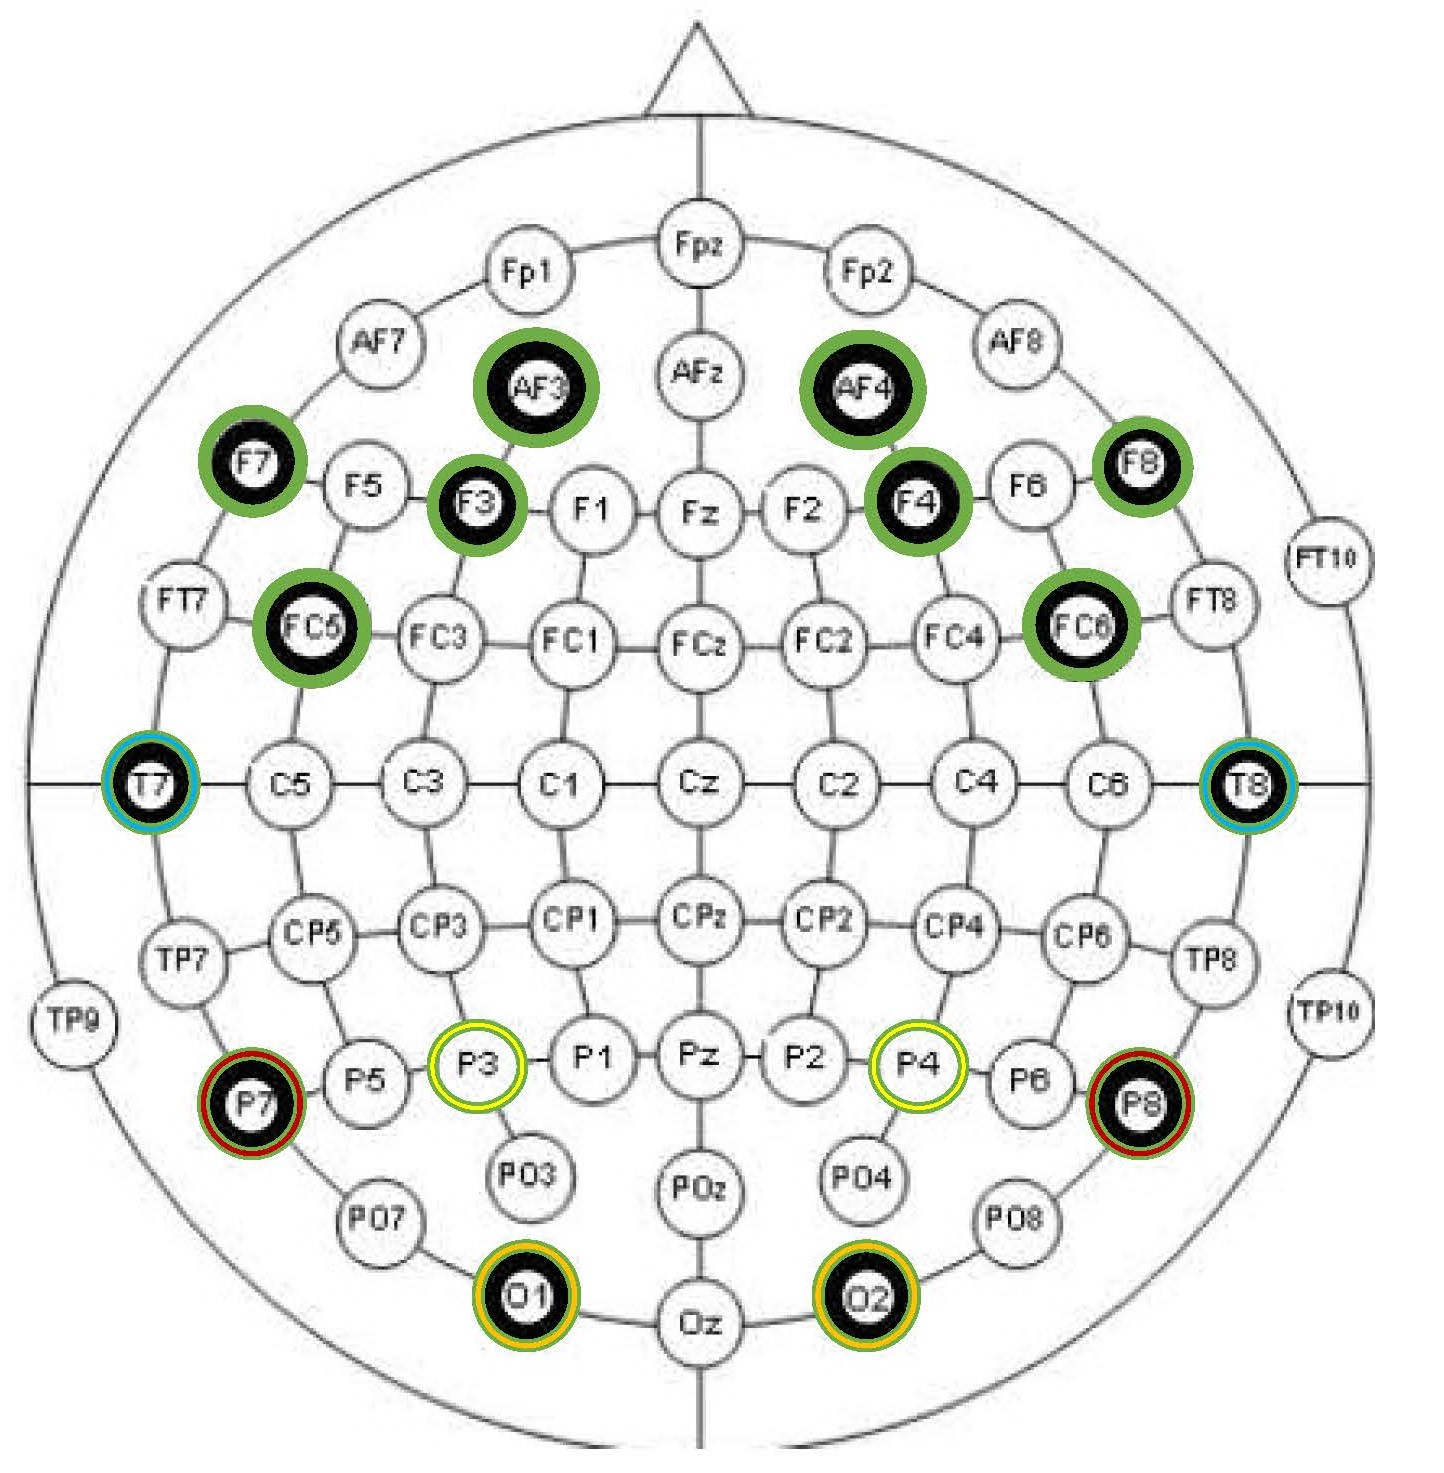
\includegraphics[width=\textwidth]{Fig2.png}
 \caption{Location and labeling of the electrodes in emotiv according to the International 10-20 Extended System.}
 \label{fig02}
 \source{Oostenveld \& Praamstra, 200.}
 \end{minipage}%
 \qquad
 \begin{minipage}{0.45\textwidth}
 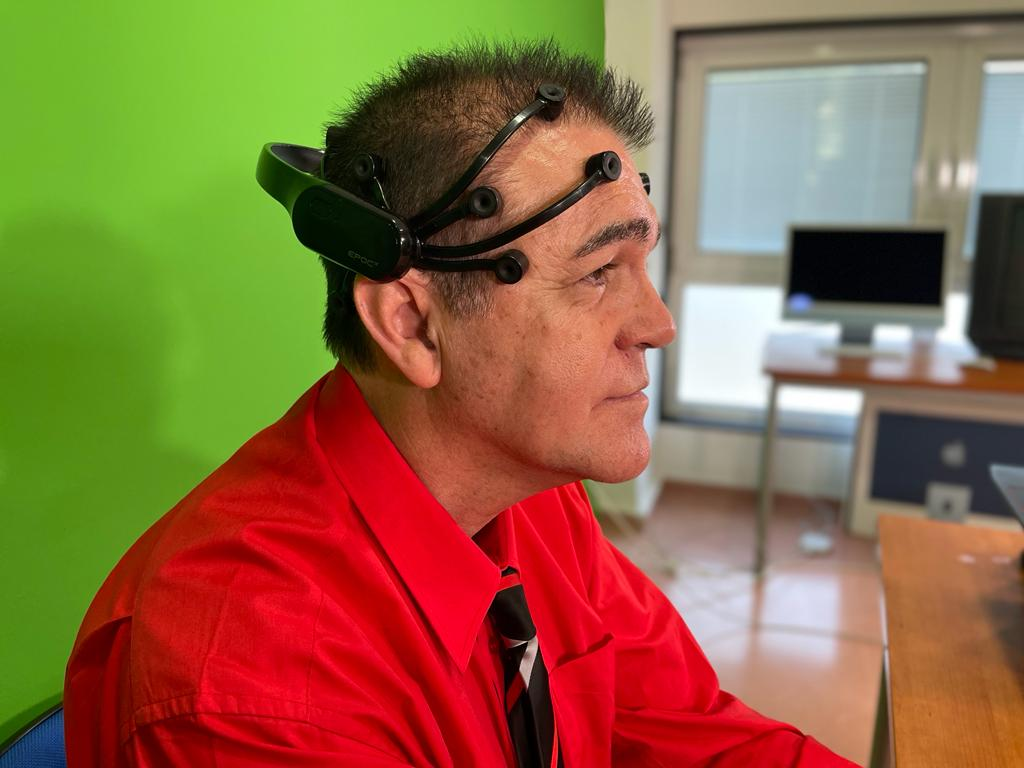
\includegraphics[width=\textwidth]{Fig3.png}
 \caption{BCI placement in the author.}
 \label{fig03}
 \source{Own elaboration.} 
 \end{minipage}%
\end{figure}

\begin{figure}[htbp]
 \centering
 \begin{minipage}{.45\textwidth}
 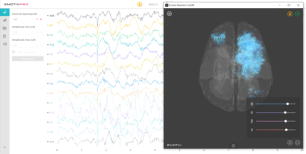
\includegraphics[width=\textwidth]{Fig4.png}
 \caption{Reading (text and images).}
 \label{fig04}
 \source{Own elaboration.}
 \end{minipage}%
 \qquad
 \begin{minipage}{0.45\textwidth}
 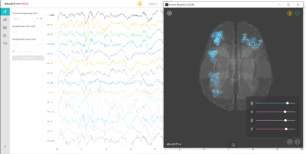
\includegraphics[width=\textwidth]{Fig5.png}
 \caption{Reading (script font).}
 \label{fig05}
 \source{Own elaboration.} 
 \end{minipage}%
\end{figure}

\begin{figure}[htbp]
 \centering
 \begin{minipage}{.45\textwidth}
 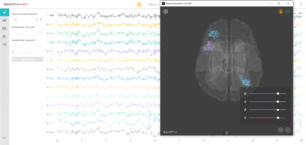
\includegraphics[width=\textwidth]{Fig6.png}
 \caption{Reading (foreign language text).}
 \label{fig06}
 \source{Own elaboration.}
 \end{minipage}%
 \qquad
 \begin{minipage}{0.45\textwidth}
 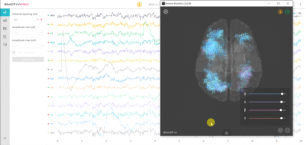
\includegraphics[width=\textwidth]{Fig7.png}
 \caption{Resolution of arithmetic operation: addition.}
 \label{fig07}
 \source{Own elaboration.} 
 \end{minipage}%
\end{figure}

\begin{figure}[htbp]
 \centering
 \begin{minipage}{.45\textwidth}
 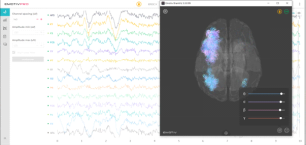
\includegraphics[width=\textwidth]{Fig8.png}
 \caption{Resolution of arithmetic operation: subtraction.}
 \label{fig08}
 \source{Own elaboration.}
 \end{minipage}%
 \qquad
 \begin{minipage}{0.45\textwidth}
 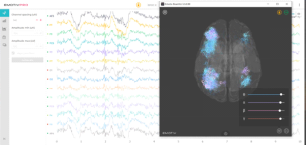
\includegraphics[width=\textwidth]{Fig9.png}
 \caption{Resolution of arithmetic operation: multiplication.}
 \label{fig09}
 \source{Own elaboration.} 
 \end{minipage}%
\end{figure}

\begin{figure}[htbp]
 \centering
 \begin{minipage}{.45\textwidth}
 
\includegraphics[width=\textwidth]{Fig10.png}
 \caption{Resolution of arithmetic operation: division.}
 \label{fig10}
 \source{Own elaboration.}
 \end{minipage}%
 \qquad
 \begin{minipage}{0.45\textwidth}
 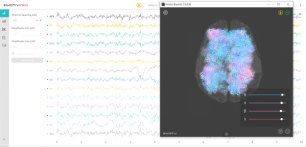
\includegraphics[width=\textwidth]{Fig11.png}
 \caption{Resolution of a mathematical problem.}
 \label{fig11}
 \source{Own elaboration.} 
 \end{minipage}%
\end{figure}

In a first approximation, without this being a generalizable result, we can say that in (\Cref{fig04}), the involvement of the right hemisphere is not a facilitator for the reading process, which is located in the left hemisphere. In (\Cref{fig04}) we observe that the neural network is fulfilled (briefly: occipital lobe - wernicke's area - angular gyrus - frontal lobe, and involvement of the right hemisphere). When the student is subjected to a reading task in a language he does not know, the corresponding neurodidactic reading network is not activated, so we have a practical application, to see live if a student is following the correct neural network in his pedagogical process of reading.

Regarding mathematics, the resolution of an addition (\Cref{fig07}), activates the frontal, parietal, temporal and left occipital lobe, as well as the right frontal and occipital lobe However, in (\Cref{fig08}) we can see that the neural activity is very different, as it happens with multiplication, division, and especially with the resolution of a problem, the question would be, do we know the neudidactic networks of each pedagogical process? Do future teachers and in-service teachers have knowledge of these networks in their initial and postgraduate training courses? This is the line of research that we are developing and that we will publish shortly.

In a second approximation, it should be noted that the tasks developed have not been performed in an artificial context, but in a natural environment, quickly and effectively, without artifices or equipment that hinder their development in the classroom (the BCI is portable), so that the neuroimaging obtained corresponds to their daily life, to the usual pedagogical context of the teacher and the student. On the other hand, the teacher can observe, in real time, the functioning of her student's brain, and although she does not have the necessary neuroscientific knowledge, she can appreciate the great usefulness of neuroimaging as the neuropedagogue "translates" what is happening in her student's brain at that very moment.

\section{Discussion and conclusions}\label{sec-modelo}
The research presented here provides a very interesting result, we are talking about the first questionnaire validated in its construct, which relates neuropedagogy with neuroeducation, neurodidactics and teacher training. The exploratory factor analysis also highlights the importance of teacher training in practical and theoretical neuropedagogical aspects. On the other hand, the correlation analysis between dimensions establishes the links between them, so that we can say that there is a significant relationship between neuroeducation and neuropedagogy, and between the latter and neurodidactics; finally, teacher training is closely related to neuroeducation. Finally, an automatic linear modeling has been performed, trying to analyze the interaction between variables and to make a prediction about the behavior of these variables, this way, we can find which variables will influence neuropedagogy to develop adequately. Regression modeling establishes that: 1) the most important aspect in neuropedagogy is the support of comparative and differential neuroeducation; 2) in decreasing order, it is key to study the human being in its educational facet in a neuroscientific way, the instructional application of neurodidactics, equally important is neuro-orientation and educational neuro-organization; 3) neuropedagogy must include the theory of education and sociology, as well as the need for training of trainers in neuropedagogy. The examples of neuroimaging, carried out from the neuropedagogical perspective, is evidence of the importance of neuroimaging for teachers, both for their daily activity, university and under and post-graduate training, supporting the present research, and serving as a starting point for further research that is already being carried out at the Universities of Jaén, Granada and the Autonomous University of Madrid.

Following \textcite{bejar_neuroeducacion_2014}, neuroeducation is configured as a branch of education, which links knowledge based on neuroimaging with the way the brain interacts with its environment. Neuropedagogy studies the pedagogical processes of students and teachers in the natural context of the educational process. We can conclude by saying that neuropedagogy is the science that studies education from a neuroeducational perspective, with the aim of configuring the neurotheory and neuromethodology of education, as well as the practical version that is neurodidactics. Neuroimaging becomes a fundamental element in neuropedagogical research, leaving, finally, the evidence of the need to implement in the studies of the Degree of Pedagogy, Degree of Early Childhood and Primary Education, and even the Degree of Social Education, the subject of "Neuropedagogy", as a fundamental basis for the training of a future teacher, typical of the XXI century.

\section{Acknowledgment}
"Formación del Profesorado Universitario en TIC Como Apoyo al Alumnado con Discapacidad". Type of Project/Grant: State Plan 2017-2023 Challenges - R+D+i Projects. Referencia: PID2019-108230RB-I00.

Included in the Ibero-American Network for the Development of the Professional Identity of Teachers (RED RIDIPD) (University of Jaén, Spain).

Project (2021-1-HR01-KA220-HED-000027562). Autonomous University of Madrid (Spain). Amount of the approved project: 371,219.00 EUR. Duration: 1.2.2022.-31.1.2025. EMIPE Group (Team for interdisciplinary improvement of educational practice). Autonomous University of Madrid.


\printbibliography\label{sec-bib}
% if the text is not in Portuguese, it might be necessary to use the code below instead to print the correct ABNT abbreviations [s.n.], [s.l.]
%\begin{portuguese}
%\printbibliography[title={Bibliography}]
%\end{portuguese}

\end{document}

